\chapter{Memory}

\begin{center}
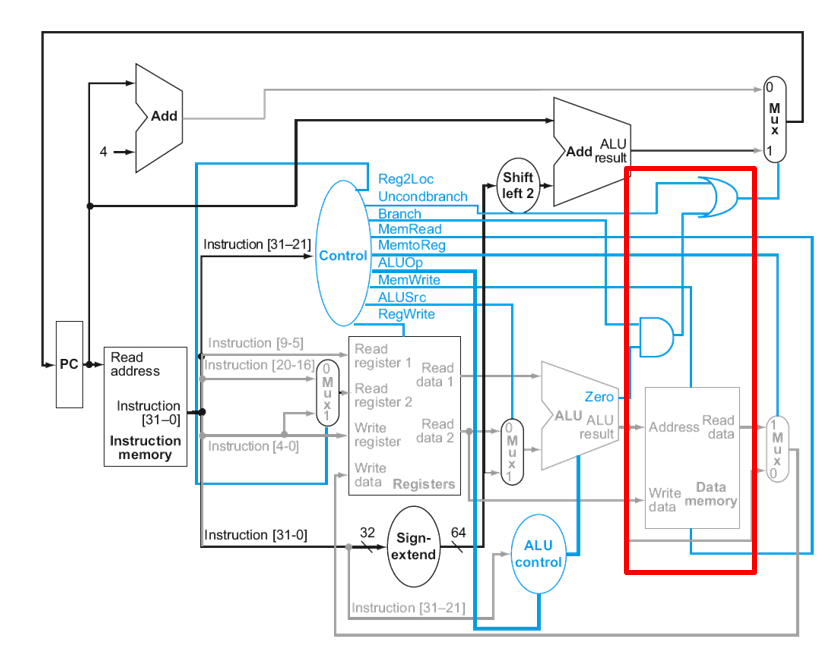
\includegraphics[width=5.5in]{../images/data_memory.png}
\end{center}


\section{Branch Resolution}

We now have all the information necessary to decide if the computer should branch or not.  We have the signal `branch' to tell us if it is a branch command, and we have `zero' to tell us if the condition was met.  Both branch and zero must be true so we will combine them with an `and' gate.

We also need an 'or' gate to 'or' together the output of the branch 'and' gate (above) and the uncondBranch control signal.  These gates can be included in your iMemory module as one line commands.  They do not need to be explicity tested, as they will be thoroughly tested when we integrate the system.  

\section{Data Memory}

This will be almost exactly like the instruction memory, with only two changes:
\begin{enumerate}
\item reading is now conditional on the `read' control wire being high.
\item writing is now permissible if the `write' control wire is high.
\end{enumerate}
As such, take your instruction memory (it is the right size, you could also use your register memory, but that would require more modification) and add the two changes above then test.

\section{Your Assignment}

You are to:
\begin{enumerate}
\item Create a new module called iMemory.
\item Instantiate the AND and OR gates directly in the iMemory stage.
\item Use instruction memory as a basis for a data memory module, and add the two new changes.  Also create or modify a fibD.data file.
\item Integrate data memory and the buffer into the iMemory stage.  
\item Write a testbench to verify that it works properly. Use a combination of fibD.data and testbench to test various scenarios.
\item There will not be a submittal for this lab.
\end{enumerate} 